% !TeX spellcheck = en_GB


%% imeko-bare-article.tex
%%% ACTA IMEKO Journal Template for submission
%%
%% Copyright (c) 2024 Federico Tramarin
%% 
%%*************************************************************************
%% Legal Notice:
%% This code is offered as-is without any warranty either expressed or
%% implied; without even the implied warranty of MERCHANTABILITY or
%% FITNESS FOR A PARTICULAR PURPOSE! 
%% User assumes all risk.
%% In no event shall the Acta Imeko or any contributor to this code be liable for
%% any damages or losses, including, but not limited to, incidental,
%% consequential, or any other damages, resulting from the use or misuse
%% of any information contained here.
%% All comments are the opinions of their respective authors and are not
%% necessarily endorsed by the Acta Imeko or Imeko.
%
% This work may be distributed and/or modified under the
% conditions of the LaTeX Project Public License, either version 1.3
% of this license or (at your option) any later version.
% The latest version of this license is in
%   https://www.latex-project.org/lppl.txt
% and version 1.3c or later is part of all distributions of LaTeX
% version 2008 or later.
%
% This work has the LPPL maintenance status `maintained'.
% 
% The Current Maintainer of this work is Federico Tramarin.
%
% This work consists of the files imeko_acta.cls, imeko_acta.bst
% and the derived file imeko_acta_template.tex and guide.tex
%
%% Retain all contribution notices and credits.
%% ** Modified files should be clearly indicated as such, including  **
%% ** renaming them and changing author support contact information. **
%%*************************************************************************

\documentclass[onecolumn,notitlepage]{article}

\begin{document}



\title{Bare Template for starting writing your own Acta IMEKO paper} % Article title

\author{Federico}

%	ABSTRACT - length less than 200 words. 
%---------------------------------------------------------------
\begin{abstract}
    The editorial team of Acta IMEKO strongly encourages 
    authors to use this \LaTeXe template file to produce their manuscript. 
    The abstract should be composed in a way suitable for publication 
    in the abstract section of electronic journals, 
    and should state concisely what it is written in the paper. 
    Important items are the aim of the research, the basic method and the major achievement 
    (also numerically, when applicable). The length should not exceed 200 words.
    \end{abstract}
    
\maketitle % Print the title and abstract box

\section{Introduction}

The introduction describes the background of the research, a 
short review of related research published in recent literature, 
together with the major claims setting the framework of the 
present publication. References should be related to the present 
publication, not just a list of papers merrily showing the authors'
knowledge of the literature. This relation must be made explicit. 
The newly presented method is shortly introduced, as an 
alternative to previously published methods, with mention of the 
advantages aimed at.


\section{First Section}

First section's text gows here.

\section{About Sections}

A further section here.

You can add figures and tables as usual.

% \begin{figure}
% 	\centering
% 	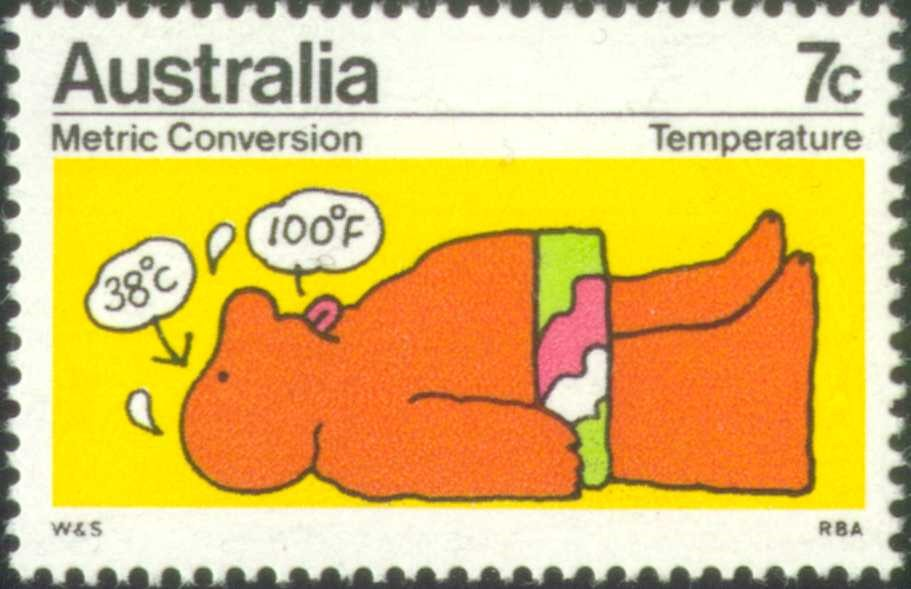
\includegraphics[width=0.68\linewidth]{image1}
% 	\caption{Stamp issued to help people getting familiar with SI units.}
% 	\label{fig:image1}
% \end{figure}

	

\subsection{Subsections} \label{sec:sub1}

If a section is long or deals with different topics, make a subdivision in subsections. Avoid further subdivision of a subsection. When subsections are used, there must be at least two. Use the style named ``Level2Title'' for the header of a subsection.

\subsection{Numbering of subsections}

Subsection numbering follows the outline numbering format which is configured in the template. Subsection headings use the Calibri font and are in bold.

\section*{acknowledgment} 

Here persons or institutes may be acknowledged for their technical, scientific or financial support. List them in this section, and not as a footnote or otherwise.


\end{document} 
